% Festlegen des Dokumententyps
\documentclass[a4paper,twoside]{article}

% Papierformat
\usepackage{a4}

% Deutsche Sprache (Silbentrennung, usw.)
\usepackage[ngerman]{babel}

% Schrifteneinstellungen
\usepackage{lmodern}
\usepackage[T1]{fontenc}
\usepackage{textcomp}

% Kodierung
\usepackage{ucs}
\usepackage[utf8]{inputenc}

% bessere Matheunterstützung
\usepackage{amsfonts}
\usepackage{amstext}
\usepackage{amsmath}

% Einheiten in Formalen
\usepackage{siunitx}

% fuer Zitate
\usepackage{cite}

% Grafiken einbinden
\usepackage{graphicx}


% Verweise in PDF-Dateien
\usepackage
[colorlinks,
pdfstartview = 1,
bookmarksopen = true,
bookmarksnumbered = true,
linkcolor = black,
plainpages = true,
hypertexnames = false,
citecolor = black]{hyperref} 

\newcommand{\e}{{\rm e}}

\begin{document}

\thispagestyle{empty}
\begin{center}
    {\Huge{\textbf{Physikalisches Praktikum}}}\\[16pt]
\ \\
\ \\
\ \\
\ \\
\ \\
\ \\
\ \\
\ \\
\ \\
\ \\
\ \\
\ \\
\ \\
\ \\
\ \\
\ \\
\ \\
\huge{Kreiselpräzession}
\ \\
\ \\
\large{Versuch 4}
\end{center}

\normalsize
\ \\
\ \\
\ \\
\ \\
\ \\

\begin{center}
\begin{tabular}{lcl}
      Name: & ~ & Timo Janßen \\
                    & ~ & E-Mail: timo.janssen1@stud.uni-goettingen.de \\
	  Mitarbeiter: & ~ & Tom Groß \\
		    & ~ & E-Mail: tom.gross@stud.uni-goettingen.de \\
\ \\		    
      Tutorin: & ~ & Jantje Freudenthal \\
      Gruppe: & ~ & 10 \\
\ \\      
      Durchgeführt am: & ~ & 27.05.2013 \\
      Protokoll abgegeben: & ~ & 10.06.2013 \\
      Protokoll verbessert: & ~ & ........................\\
\ \\
\ \\
      Testiert: .................................    
\end{tabular}\\
\end{center}

\newpage
%Seitennummerierung ausschalten
\thispagestyle{empty}
\tableofcontents
\newpage
%Seitenzähler zurücksetzen
\setcounter{page}{1}
\section{Einleitung}
In diesem Versuch geht es um die Untersuchung der Rotationen eines Kreisels und den sich daraus ergebenden Eigenschaften. Insbesondere die Präzession soll näher betrachtet werden. Kreisel sind alltägliche Gegenstände, ob als Spielzeug oder auch als Messinstrument (zum Beispiel als Gyroskop). Die Bewegungsgleichungen des Kreisels finden insbesondere in der Astronomie Anwendung, wo sie die Bewegungen der Himmelskörper beschreiben.
\newpage
\section{Theorie}
\subsection{Die gedämpfte erzwungene Schwingung}
In der homogenen Differentialgleichung des gedämpften harmonischen Oszillators gibt es drei wesentliche Größen: Das der
(Winkel-)Beschleunigung entgegenwirkende Trägheitsmoment $\Theta$ (hier das Schwungrad), die zur (Winkel-)Geschwindigkeit proportionale Reibung
$\rho$ und das direkt zur Position (hier der Winkel $\phi$) proportionale Rückstellmoment $D^*$.
Hinzu kommt die Anregung. Diese wird periodisch beschrieben durch $M\cos(\omega t).$ 
Zusammen ergeben diese Faktoren die Bewegungsgleichung des Pohlschen Rades:
\begin{align}
\label{eq:1}
\Theta\ddot{\varphi}+\rho\dot{\varphi}+D^*=M\cos(\omega t)
\end{align}
Um diese Gleichung auf die Normalform einer Bewegungsgleichung für eine gedämpfte Schwingung mit Anregung zu bringen, teilen
wir durch $\Theta$ und erhalten für $\rho/\Theta=:2\beta$, $D^*/\Theta=:\omega_0^2$ und $M/\Theta=:N$
die inhomogene lineare Differentialgleichung 2. Ordnung
\begin{align}
\label{eq:2}
\ddot{\varphi}+2\beta\dot{\varphi}+\omega_0^2\varphi=N\cos(\omega t).
\end{align}


\subsection{Die homogene Differentialgleichung}
\label{h.DGL}
Betrachten wir zunächst die Gleichung des frei schwingenden Rades, also ohne Anregung, so erhalten wir die homogene Differentialgleichung
\begin{align}
\label{eq:3}
\ddot{\varphi}+2\beta\dot{\varphi}+\omega_0^2\varphi=0
\end{align}
welche mit dem Exponentialansatz $\varphi(t)=e^{\lambda t}$ gelöst werden kann. Hier sind die drei Fälle $\beta>\omega_0$, $\beta=\omega_0$ und $\beta<\omega_0$ zu unterscheiden. 
Wir werden uns hier mit dem sogenannten Schwingfall $\beta<\omega_0$ befassen. 
Offensichtlich bekommt hier die Wurzel ein negatives Argument, was zu folgender Lösung für
Gleichung (\ref{eq:3}) führt:
\begin{align}
\label{eq:4}
\varphi(t)=e^{-\beta t}\cdot\left(Ae^{i\sqrt{\omega_0^2-\beta^2}t} + Be^{-i\sqrt{\omega_0^2-\beta^2}t}\right)
\end{align}
Nun ist noch die Anfangsphase $\phi$, sowie die Reellen Zahlen A und B, welche 
in der Ausgangsamplitude $\varphi_0$ zusammengefasst werden zu bestimmen. Setzen wir $A:=\frac{\varphi_0}{2}\cdot e^{i\phi}$ und 
$B:=\frac{\varphi_0}{2}\cdot e^{-i\phi}=\bar{A}$ so erhalten wir \begin{align}
\label{eq:5}
\varphi(t) &= e^{-\beta t}\cdot\left(\frac{\varphi_0}{2}\cdot e^{i\phi}\cdot e^{i\sqrt{\omega_0^2-\beta^2}t} + 
\frac{\varphi_0}{2}\cdot e^{-i\phi}\cdot e^{-i\sqrt{\omega_0^2-\beta^2}t}\right)\nonumber \\
&= e^{-\beta t}\cdot\frac{\varphi_0}{2}\cdot\left(e^{i(\phi+\sqrt{\omega_0^2-\beta^2}t)}+e^{-i(\phi+\sqrt{\omega_0^2-\beta^2}t)}\right).
\end{align}
Mit $\sqrt{\omega_0^2-\beta^2}=:\omega_e$, der Eigenfrequenz des Rades bei der entsprechenden Schwingung, folgt nach der 
\glqq Eulerschen Identität \grqq{} die Schwingungsgleichung für das Pohlsche Rad ohne Antrieb.
\begin{align}
\label{eq:6}
\varphi(t)=\varphi_0\cdot e^{\beta t}\cdot\cos(\omega_e + \phi)
\end{align}

\subsection{Interpretation und logarithmisches Dekrement}
\label{log.Dek}
Der Schwingungsverlauf des Rades ist also cosinus-periodisch und wird um den von der Zeit abhängigen Faktor $e^{-\beta t}$ geschwächt. 
Diese  Dämpfung kann über das logarithmische Dekrement $\Lambda$ beschrieben werden. Dabei gilt:
\begin{align}
\label{eq:7}
\Lambda := \rm {ln}\left[{\frac{\varphi(t)}{\varphi(t+T)}}\right]={\rm {ln}}[e^{\beta T}]=\beta T
\end{align}
Hier beschreibt T die Periodendauer. Das logarithmische Dekrement hängt also lediglich von der Periodendauer, nicht 
von der Zeit ab.

\subsection{Die inhomogene Differentialgleichung}
\label{inh.DGL}
Um die Gleichung der erzwungenen Schwingung zu finden, müssen wir nun die inhomogene Gleichung (\ref{eq:2}) lösen. 
Die Lösung einer inhomogenen Gleichung setzt sich aus der Lösung der zugehörigen homogenen 
Differentialgleichung (\ref{eq:6}) und einer partikulären Lösung zusammen. 
Die partikuläre Lösung erhalten wir durch Einsetzen des Ansatzes $\varphi=\varphi_0\cdot \cos(\omega t-\phi)+c$ in 
(\ref{eq:2}):
\begin{align}
\label{eq:8}
(\omega_0^2-\omega^2)\cdot\varphi_0\cdot\cos(\omega t-\phi)-2\beta\cdot\omega\cdot\sin(\omega t-\phi)+c=N\cos(\omega t). 
\end{align}
Nun müssen $\varphi_0$ und $\phi$ so bestimmt werden, dass die Gleichung für alle Zeiten t erfüllt ist.
Mithilfe der Additionstheoreme gelangt man von dieser Gleichung zu folgenden zwei Bedingungen:
\begin{align}
\label{eq:9}
\varphi_0\cdot\left((\omega_0^2-\omega^2)\cdot\cos(\phi)+2\beta\cdot\omega\cdot\sin(\phi)\right) &= N \\
\label{eq:10}
(\omega_0^2-\omega^2\cdot\sin(\phi) &= 2\beta\cdot\omega\cdot\cos(\phi)
\end{align}
Aus (\ref{eq:10}) folgt direkt die Phasenverschiebung:
\begin{align}
\label{eq:11}
\phi=\arctan\left(\frac{2\beta\omega}{\omega_0^2-\omega^2}\right)
\end{align}
Aus (\ref{eq:9}) lässt sich nach kurzem Umformen und Einsetzen der Phasenverschiebung $\varphi_0$ bestimmen:
\begin{align}
\label{eq:12}
\varphi_0=\frac{N}{(\omega_0^2-\omega^2)^+4\beta^2\cdot\omega^2}
\end{align}
Einsetzen dieses Ergebnisses führt zu folgender partikuläreN Lösung der Schwingungsgleichung (\ref{eq:2}) für die gedämpfte erzwungene Schwingung 
des Pohlschen Rades:
\begin{align}
\label{eq:13}
\varphi(t)=\frac{N}{(\omega_0^2-\omega^2)^+4\beta^2\cdot\omega^2}\cdot\cos\left(\omega t-\arctan\left(\frac{2\beta\omega}{\omega_0^2-\omega^2}\right)\right)
\end{align}
Da die Lösung der homogenen Differentialgleichung für lange Messzeiten gegen Null geht (die Amplitude fällt mit der Exponentialfunktion $e^{-\beta t}$ 
ab), kann für die erzwungene Schwingung bei längeren Schwingzeiten die homogene Gleichung vernachlässigt werden.
Damit beschreibt die partikuläre Lösung der inhomogenen Differentialgleichung die Schwingung für große Zeiten t zunehmend genau. Die Zeit, nach der die homogene Gleichung mit Null angenähert werden kann bezeichnet man als Einschwingvorgang.
\newpage
\subsection{Die Amplitudengleichung}
\label{ampl}
Die Amplitudenstärke
\begin{align}
\label{eq:14}
A(\omega,\beta)=\frac{N}{(\omega_0^2-\omega^2)^2+4\beta^2\cdot\omega^2}
\end{align}
ist gegeben als Vorfaktor der Schwingungsgleichung (\ref{eq:13}) in Abhängigkeit von der Erregerfrequenz $\omega$ und der Dämpfung $\beta$.
Da wir das Resonanzverhalten der Schwingung bei einer bestimmten Dämpfung betrachten wollen, gehen wir jeweils von einem festen $\beta$ aus 
und bestimmen die Amplitude in Abhängigkeit von der Anregung.\\
Dabei ist das Betrachten des Maximums besonders relevant. Dafür berechnen wir die Nullstellen der Ableitung der 
Amplitudengleichung. Die relevante Nullstelle dieser Ableitung ist
\begin{align}
\label{eq:16}
\omega=\sqrt{\omega_0^2-2\beta^2}=:\omega_r.
\end{align}
$\omega_r$ ist die Resonanzfrequenz des Systems. Entspricht die Anregungsfrequenz der Resonanzfrequenz, des angeregten 
Systems, so wird die Schwingsamplitude maximal. In diesem Fall, wird das schwingende System immer weiter angeregt, 
bis es schließlich (abhängig von der Dämpfung) im Extremfall zu einer sogenannten Resonanzkatastrophe
kommt. Als Resonanzkatastrophe wird der Zustand bezeichnet, bei welchem die Amplitude des schwingenden Systems gegen 
unendlich geht. 

\subsection{Phasenverschiebung}
In Kapitel \ref{inh.DGL} wurde die Gleichung (\ref{eq:11}) der Phasenverschiebung
\begin{align}
\phi=\arctan\left(\frac{2\beta\omega}{\omega_0^2-\omega^2}\right) \nonumber
\end{align}
hergeleitet.
Anhand dieser Gleichung ist zu sehen, wie sich unterschiedliche Dämpfungen, beziehungsweise Anregungen auf die 
Phasenverschiebung $\phi$ auswirken.
\newpage
\section{Der Versuch}
\subsection{Versuchsaufbau}
Die Versuchsapparatur besteht im Wesentlichen aus drei Elementen: Einem Rechner mit Bildschirm, dem Pohlschen Rad mit 
Wirbelstrombremse und einem Schrittmotor mit Exzenter als externem Anreger für das Rad.

\subsection{Durchführung}
Für vier Stellungen der Wirbelstrombremse ($\SI{0}{mm}$, $\SI{4}{mm}$, $\SI{6}{mm}$ und $\SI{8}{mm}$) wird das Verhalten der freien Schwingung aufgezeichnet. Anschließend werden für die drei Stellungen der Wirbelstrombremse $\SI{4}{mm}$, $\SI{6}{mm}$ und $\SI{8}{mm}$
jeweils Messungen für Anregungsfrequenzen im Bereich von 100-600 mHz durchgeführt. Insbesondere werden hier zusätzliche 
Messungen in der Umgebung der Resonanzfrequenz aufgezeichnet.\\
Bei der Messung der Schwingung mit Anregung ist es wichtig, die Einschwingzeit (vgl. Kap. \ref{inh.DGL}) zu berücksichtigen, um eine Verfälschung der 
Messdaten zu verhindern. Besondere Vorsicht ist bei Messungen nahe der Resonanzfrequenz (vgl. Kap. \ref{ampl}) geboten. Außerdem ist es für die
Auswertung des Versuches wichtig, hinreichend viele Messungen insbesondere um den Resonanzbereich zu tätigen, da sonst der 
Verlauf in diesem Bereich nur sehr ungenau dargestellt werden kann.


\newpage
\section{Auswertung}
\subsection{Schwingungen ohne Anregungen}
Nach der Aufbereitung der Messdaten kann zunächst der zeitliche Verlauf der nicht angeregten Schwingung für die verschiedenen Dämpfungen dargestellt werden (Abb. \ref{img:1}). Man erkennt deutlich das schnellere Abklingen bei stärkerer Dämpfung. 
Die Eigenfrequenz dieser Schwingungen bestimmt sich als Maximum der zugehörigen diskreten Fourier-Transformation (DFT) ~\cite[Rao, 2010]{FFT}. Die Ergebnisse sind in Tabelle \ref{tab:1} aufgetragen.
\begin{figure}[!htbp]
\centering
   % GNUPLOT: LaTeX picture with Postscript
\begingroup
  \makeatletter
  \providecommand\color[2][]{%
    \GenericError{(gnuplot) \space\space\space\@spaces}{%
      Package color not loaded in conjunction with
      terminal option `colourtext'%
    }{See the gnuplot documentation for explanation.%
    }{Either use 'blacktext' in gnuplot or load the package
      color.sty in LaTeX.}%
    \renewcommand\color[2][]{}%
  }%
  \providecommand\includegraphics[2][]{%
    \GenericError{(gnuplot) \space\space\space\@spaces}{%
      Package graphicx or graphics not loaded%
    }{See the gnuplot documentation for explanation.%
    }{The gnuplot epslatex terminal needs graphicx.sty or graphics.sty.}%
    \renewcommand\includegraphics[2][]{}%
  }%
  \providecommand\rotatebox[2]{#2}%
  \@ifundefined{ifGPcolor}{%
    \newif\ifGPcolor
    \GPcolortrue
  }{}%
  \@ifundefined{ifGPblacktext}{%
    \newif\ifGPblacktext
    \GPblacktexttrue
  }{}%
  % define a \g@addto@macro without @ in the name:
  \let\gplgaddtomacro\g@addto@macro
  % define empty templates for all commands taking text:
  \gdef\gplbacktext{}%
  \gdef\gplfronttext{}%
  \makeatother
  \ifGPblacktext
    % no textcolor at all
    \def\colorrgb#1{}%
    \def\colorgray#1{}%
  \else
    % gray or color?
    \ifGPcolor
      \def\colorrgb#1{\color[rgb]{#1}}%
      \def\colorgray#1{\color[gray]{#1}}%
      \expandafter\def\csname LTw\endcsname{\color{white}}%
      \expandafter\def\csname LTb\endcsname{\color{black}}%
      \expandafter\def\csname LTa\endcsname{\color{black}}%
      \expandafter\def\csname LT0\endcsname{\color[rgb]{1,0,0}}%
      \expandafter\def\csname LT1\endcsname{\color[rgb]{0,1,0}}%
      \expandafter\def\csname LT2\endcsname{\color[rgb]{0,0,1}}%
      \expandafter\def\csname LT3\endcsname{\color[rgb]{1,0,1}}%
      \expandafter\def\csname LT4\endcsname{\color[rgb]{0,1,1}}%
      \expandafter\def\csname LT5\endcsname{\color[rgb]{1,1,0}}%
      \expandafter\def\csname LT6\endcsname{\color[rgb]{0,0,0}}%
      \expandafter\def\csname LT7\endcsname{\color[rgb]{1,0.3,0}}%
      \expandafter\def\csname LT8\endcsname{\color[rgb]{0.5,0.5,0.5}}%
    \else
      % gray
      \def\colorrgb#1{\color{black}}%
      \def\colorgray#1{\color[gray]{#1}}%
      \expandafter\def\csname LTw\endcsname{\color{white}}%
      \expandafter\def\csname LTb\endcsname{\color{black}}%
      \expandafter\def\csname LTa\endcsname{\color{black}}%
      \expandafter\def\csname LT0\endcsname{\color{black}}%
      \expandafter\def\csname LT1\endcsname{\color{black}}%
      \expandafter\def\csname LT2\endcsname{\color{black}}%
      \expandafter\def\csname LT3\endcsname{\color{black}}%
      \expandafter\def\csname LT4\endcsname{\color{black}}%
      \expandafter\def\csname LT5\endcsname{\color{black}}%
      \expandafter\def\csname LT6\endcsname{\color{black}}%
      \expandafter\def\csname LT7\endcsname{\color{black}}%
      \expandafter\def\csname LT8\endcsname{\color{black}}%
    \fi
  \fi
  \setlength{\unitlength}{0.0500bp}%
  \begin{picture}(7200.00,5040.00)%
    \gplgaddtomacro\gplbacktext{%
      \csname LTb\endcsname%
      \put(948,3066){\makebox(0,0)[r]{\strut{}-1}}%
      \csname LTb\endcsname%
      \put(948,3360){\makebox(0,0)[r]{\strut{}-0.5}}%
      \csname LTb\endcsname%
      \put(948,3654){\makebox(0,0)[r]{\strut{}0}}%
      \csname LTb\endcsname%
      \put(948,3947){\makebox(0,0)[r]{\strut{}0.5}}%
      \csname LTb\endcsname%
      \put(948,4241){\makebox(0,0)[r]{\strut{}1}}%
      \csname LTb\endcsname%
      \put(1080,2552){\makebox(0,0){\strut{}}}%
      \csname LTb\endcsname%
      \put(1656,2552){\makebox(0,0){\strut{}}}%
      \csname LTb\endcsname%
      \put(2232,2552){\makebox(0,0){\strut{}}}%
      \csname LTb\endcsname%
      \put(2807,2552){\makebox(0,0){\strut{}}}%
      \csname LTb\endcsname%
      \put(3383,2552){\makebox(0,0){\strut{}}}%
      \put(178,3653){\rotatebox{-270}{\makebox(0,0){\strut{}$\varphi/\varphi_0$}}}%
    }%
    \gplgaddtomacro\gplfronttext{%
      \csname LTb\endcsname%
      \put(2972,4362){\makebox(0,0)[r]{\strut{}Dämpfung 0mm}}%
    }%
    \gplgaddtomacro\gplbacktext{%
      \csname LTb\endcsname%
      \put(3828,3066){\makebox(0,0)[r]{\strut{}}}%
      \csname LTb\endcsname%
      \put(3828,3360){\makebox(0,0)[r]{\strut{}}}%
      \csname LTb\endcsname%
      \put(3828,3654){\makebox(0,0)[r]{\strut{}}}%
      \csname LTb\endcsname%
      \put(3828,3947){\makebox(0,0)[r]{\strut{}}}%
      \csname LTb\endcsname%
      \put(3828,4241){\makebox(0,0)[r]{\strut{}}}%
      \csname LTb\endcsname%
      \put(3960,2552){\makebox(0,0){\strut{}}}%
      \csname LTb\endcsname%
      \put(4536,2552){\makebox(0,0){\strut{}}}%
      \csname LTb\endcsname%
      \put(5112,2552){\makebox(0,0){\strut{}}}%
      \csname LTb\endcsname%
      \put(5687,2552){\makebox(0,0){\strut{}}}%
      \csname LTb\endcsname%
      \put(6263,2552){\makebox(0,0){\strut{}}}%
    }%
    \gplgaddtomacro\gplfronttext{%
      \csname LTb\endcsname%
      \put(5852,4362){\makebox(0,0)[r]{\strut{}Dämpfung 4mm}}%
    }%
    \gplgaddtomacro\gplbacktext{%
      \csname LTb\endcsname%
      \put(948,1302){\makebox(0,0)[r]{\strut{}-1}}%
      \csname LTb\endcsname%
      \put(948,1596){\makebox(0,0)[r]{\strut{}-0.5}}%
      \csname LTb\endcsname%
      \put(948,1890){\makebox(0,0)[r]{\strut{}0}}%
      \csname LTb\endcsname%
      \put(948,2183){\makebox(0,0)[r]{\strut{}0.5}}%
      \csname LTb\endcsname%
      \put(948,2477){\makebox(0,0)[r]{\strut{}1}}%
      \csname LTb\endcsname%
      \put(1080,788){\makebox(0,0){\strut{}0}}%
      \csname LTb\endcsname%
      \put(1656,788){\makebox(0,0){\strut{}5}}%
      \csname LTb\endcsname%
      \put(2232,788){\makebox(0,0){\strut{}10}}%
      \csname LTb\endcsname%
      \put(2807,788){\makebox(0,0){\strut{}15}}%
      \csname LTb\endcsname%
      \put(3383,788){\makebox(0,0){\strut{}20}}%
      \put(178,1889){\rotatebox{-270}{\makebox(0,0){\strut{}$\varphi/\varphi_0$}}}%
      \put(2519,458){\makebox(0,0){\strut{}$t [s]$}}%
    }%
    \gplgaddtomacro\gplfronttext{%
      \csname LTb\endcsname%
      \put(2972,2598){\makebox(0,0)[r]{\strut{}Dämpfung 6mm}}%
    }%
    \gplgaddtomacro\gplbacktext{%
      \csname LTb\endcsname%
      \put(3828,1302){\makebox(0,0)[r]{\strut{}}}%
      \csname LTb\endcsname%
      \put(3828,1596){\makebox(0,0)[r]{\strut{}}}%
      \csname LTb\endcsname%
      \put(3828,1890){\makebox(0,0)[r]{\strut{}}}%
      \csname LTb\endcsname%
      \put(3828,2183){\makebox(0,0)[r]{\strut{}}}%
      \csname LTb\endcsname%
      \put(3828,2477){\makebox(0,0)[r]{\strut{}}}%
      \csname LTb\endcsname%
      \put(3960,788){\makebox(0,0){\strut{}0}}%
      \csname LTb\endcsname%
      \put(4536,788){\makebox(0,0){\strut{}5}}%
      \csname LTb\endcsname%
      \put(5112,788){\makebox(0,0){\strut{}10}}%
      \csname LTb\endcsname%
      \put(5687,788){\makebox(0,0){\strut{}15}}%
      \csname LTb\endcsname%
      \put(6263,788){\makebox(0,0){\strut{}20}}%
      \put(5399,458){\makebox(0,0){\strut{}$t [s]$}}%
    }%
    \gplgaddtomacro\gplfronttext{%
      \csname LTb\endcsname%
      \put(5852,2598){\makebox(0,0)[r]{\strut{}Dämpfung 8mm}}%
    }%
    \gplbacktext
    \put(0,0){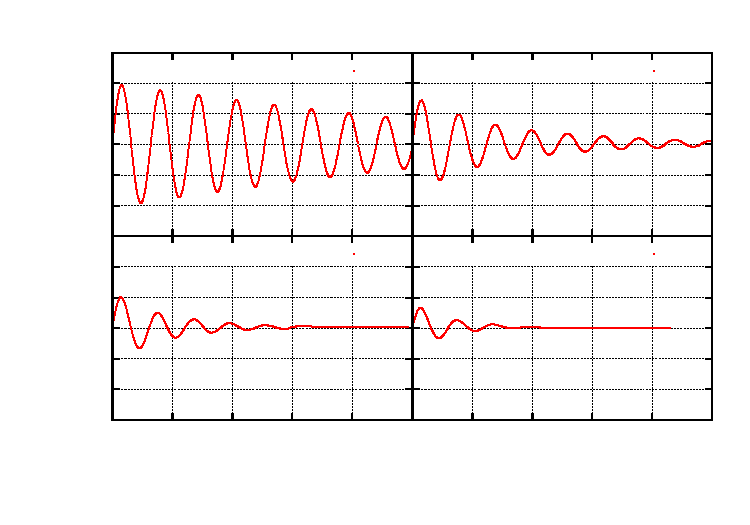
\includegraphics{plot_dif0}}%
    \gplfronttext
  \end{picture}%
\endgroup

   \caption{\small{Schwingungsverlauf des Pohlschen Rades ohne Anregung für vier verschiedene Dämpfungen}}
   \label{img:1}
\end{figure}
\ \\
Mit der Gleichung
\begin{align}
\Lambda := \rm {ln}\left[{\frac{\varphi(t)}{\varphi(t+T)}}\right]=\beta T \nonumber
\end{align}
kann das Logarithmische Dekrement berechnet werden. Dazu werden mit einem Peakfinding-Algorithmus die Maxima der Schwingung bestimmt und jeweils für zwei benachbarte Maxima das Logarithmische Dekrement berechnet. Anschließend werden die Werte gemittelt. Die Dämpfung $\beta$ ergibt sich dann durch Multiplikation mit der Periodendauer. Die Ergebnisse befinden sich ebenfalls in Tabelle \ref{tab:1}.\\
Damit lässt sich nun die ungedämpfte Eigenfrequenz über die Beziehung
\begin{align}
\omega_e = \sqrt{\omega_0^{2}-\beta^{2}}  \Leftrightarrow \omega_0 = \sqrt{\omega_e^{2}+\beta^{2}}
\end{align}
finden. Der Mittelwert über die vier Messungen ist
\begin{align}
\omega_0 = \SI{2,08\pm0,18}{\per\second} \nonumber
\end{align}
Dieser stimmt nicht überein mit der Eigenfrequenz für die Stellung "`0 mm"' der Wirbelstrombremse. Dies ist aber nicht verwunderlich, wenn man bedenkt, dass das betrachtete System selbst bei abgeschalteter Wirbelstrombremse nicht völlig reibungs- bzw. dämpfungsfrei ist. Es treten sowohl Luftreibung, als auch mechanische Reibung in den Lagern auf, was sich auch im Wert der Dämpfungskonstante niederschlägt.
\begin{table}[!htbp]
\centering
\begin{tabular}{|l|l|l|l|l|}
\hline 
Dämpfung & $\SI{0}{mm}$ & $\SI{4}{mm}$ & $\SI{6}{mm}$ & $\SI{8}{mm}$ \\
\hline
$\omega_e$ $[\SI{}{\per\second}]$ & $\SI{2,06\pm0,10}{\per\second}$ & $\SI{2,06\pm0,10}{\per\second}$ & $\SI{2,16\pm0,13}{\per\second}$ & $\SI{1,96\pm0,15}{\per\second}$ \\
\hline
$\Lambda$ & $\SI{0,112\pm0,005}{}$ & $\SI{0,38\pm0,06}{}$ & $\SI{0,80\pm0,06}{}$ & $\SI{1,5\pm0,4}{}$ \\
\hline
$\beta$ $[\SI{}{\per\second}]$ & \SI{0,037\pm0,005}{} & \SI{0,12\pm0,06}{} & \SI{0,27\pm0,06}{} & \SI{0,5\pm0,4}{} \\
%\hline
%Errechnete & & & & \\ ungedämpfte & & & & \\  Eigenfrequenz & & & & \\$\omega_0$: & ... & ... & ... & \\
\hline 
\end{tabular} 
\caption{\small{Auswertung der Schwingungen für die vier Dämpfungen ohne Anregung}}
\label{tab:1}
\end{table}
\newpage
\subsection{Schwingungen mit Anregungen}
Zunächst soll für jede Dämpfung die Resonanzkurve aufgetragen werden. Dazu  muss für jede Kombination aus Dämpfung und Erregerfrequenz die Schwingungsamplitude bestimmt werden. Dies geschieht durch Suchen der Minima/Maxima mit dem bereits erwähnten Peakfinding-Algorithmus und anschließende Mittelwertbildung. Abbildung \ref{img:2} zeigt die resultierenden Kurven für alle Dämpfungen:
\ \\
\begin{figure}[!htbp]
\centering
% GNUPLOT: LaTeX picture with Postscript
\begingroup
  \makeatletter
  \providecommand\color[2][]{%
    \GenericError{(gnuplot) \space\space\space\@spaces}{%
      Package color not loaded in conjunction with
      terminal option `colourtext'%
    }{See the gnuplot documentation for explanation.%
    }{Either use 'blacktext' in gnuplot or load the package
      color.sty in LaTeX.}%
    \renewcommand\color[2][]{}%
  }%
  \providecommand\includegraphics[2][]{%
    \GenericError{(gnuplot) \space\space\space\@spaces}{%
      Package graphicx or graphics not loaded%
    }{See the gnuplot documentation for explanation.%
    }{The gnuplot epslatex terminal needs graphicx.sty or graphics.sty.}%
    \renewcommand\includegraphics[2][]{}%
  }%
  \providecommand\rotatebox[2]{#2}%
  \@ifundefined{ifGPcolor}{%
    \newif\ifGPcolor
    \GPcolortrue
  }{}%
  \@ifundefined{ifGPblacktext}{%
    \newif\ifGPblacktext
    \GPblacktexttrue
  }{}%
  % define a \g@addto@macro without @ in the name:
  \let\gplgaddtomacro\g@addto@macro
  % define empty templates for all commands taking text:
  \gdef\gplbacktext{}%
  \gdef\gplfronttext{}%
  \makeatother
  \ifGPblacktext
    % no textcolor at all
    \def\colorrgb#1{}%
    \def\colorgray#1{}%
  \else
    % gray or color?
    \ifGPcolor
      \def\colorrgb#1{\color[rgb]{#1}}%
      \def\colorgray#1{\color[gray]{#1}}%
      \expandafter\def\csname LTw\endcsname{\color{white}}%
      \expandafter\def\csname LTb\endcsname{\color{black}}%
      \expandafter\def\csname LTa\endcsname{\color{black}}%
      \expandafter\def\csname LT0\endcsname{\color[rgb]{1,0,0}}%
      \expandafter\def\csname LT1\endcsname{\color[rgb]{0,1,0}}%
      \expandafter\def\csname LT2\endcsname{\color[rgb]{0,0,1}}%
      \expandafter\def\csname LT3\endcsname{\color[rgb]{1,0,1}}%
      \expandafter\def\csname LT4\endcsname{\color[rgb]{0,1,1}}%
      \expandafter\def\csname LT5\endcsname{\color[rgb]{1,1,0}}%
      \expandafter\def\csname LT6\endcsname{\color[rgb]{0,0,0}}%
      \expandafter\def\csname LT7\endcsname{\color[rgb]{1,0.3,0}}%
      \expandafter\def\csname LT8\endcsname{\color[rgb]{0.5,0.5,0.5}}%
    \else
      % gray
      \def\colorrgb#1{\color{black}}%
      \def\colorgray#1{\color[gray]{#1}}%
      \expandafter\def\csname LTw\endcsname{\color{white}}%
      \expandafter\def\csname LTb\endcsname{\color{black}}%
      \expandafter\def\csname LTa\endcsname{\color{black}}%
      \expandafter\def\csname LT0\endcsname{\color{black}}%
      \expandafter\def\csname LT1\endcsname{\color{black}}%
      \expandafter\def\csname LT2\endcsname{\color{black}}%
      \expandafter\def\csname LT3\endcsname{\color{black}}%
      \expandafter\def\csname LT4\endcsname{\color{black}}%
      \expandafter\def\csname LT5\endcsname{\color{black}}%
      \expandafter\def\csname LT6\endcsname{\color{black}}%
      \expandafter\def\csname LT7\endcsname{\color{black}}%
      \expandafter\def\csname LT8\endcsname{\color{black}}%
    \fi
  \fi
  \setlength{\unitlength}{0.0500bp}%
  \begin{picture}(7200.00,5040.00)%
    \gplgaddtomacro\gplbacktext{%
      \csname LTb\endcsname%
      \put(682,704){\makebox(0,0)[r]{\strut{} 0}}%
      \put(682,1213){\makebox(0,0)[r]{\strut{} 1}}%
      \put(682,1722){\makebox(0,0)[r]{\strut{} 2}}%
      \put(682,2231){\makebox(0,0)[r]{\strut{} 3}}%
      \put(682,2740){\makebox(0,0)[r]{\strut{} 4}}%
      \put(682,3248){\makebox(0,0)[r]{\strut{} 5}}%
      \put(682,3757){\makebox(0,0)[r]{\strut{} 6}}%
      \put(682,4266){\makebox(0,0)[r]{\strut{} 7}}%
      \put(682,4775){\makebox(0,0)[r]{\strut{} 8}}%
      \put(814,484){\makebox(0,0){\strut{} 0}}%
      \put(2311,484){\makebox(0,0){\strut{} 0.5}}%
      \put(3809,484){\makebox(0,0){\strut{} 1}}%
      \put(5306,484){\makebox(0,0){\strut{} 1.5}}%
      \put(6803,484){\makebox(0,0){\strut{} 2}}%
      \put(176,2739){\rotatebox{-270}{\makebox(0,0){\strut{}$\phi_0(\omega)/\phi_0(0)$}}}%
      \put(3808,154){\makebox(0,0){\strut{}$\omega/\omega_0$}}%
    }%
    \gplgaddtomacro\gplfronttext{%
      \csname LTb\endcsname%
      \put(5816,4602){\makebox(0,0)[r]{\strut{}4mm}}%
      \csname LTb\endcsname%
      \put(5816,4382){\makebox(0,0)[r]{\strut{}6mm}}%
      \csname LTb\endcsname%
      \put(5816,4162){\makebox(0,0)[r]{\strut{}8mm}}%
    }%
    \gplbacktext
    \put(0,0){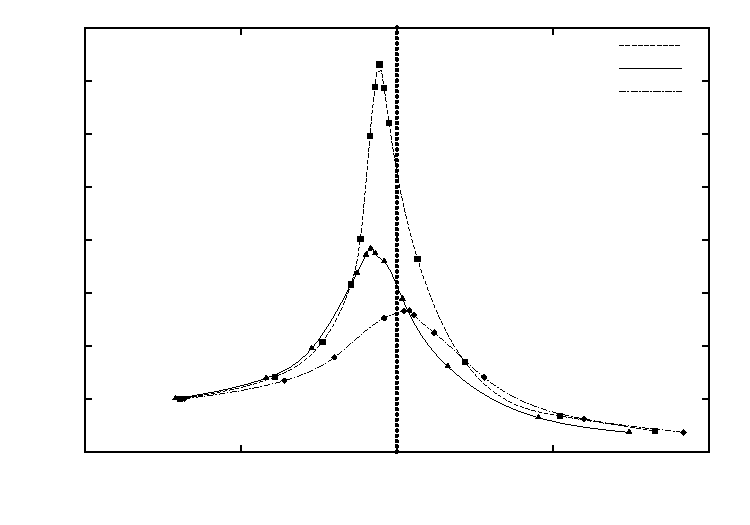
\includegraphics{frequenzgang}}%
    \gplfronttext
  \end{picture}%
\endgroup

\caption{Das unterschiedliche Resonanzverhalten des Rades für die drei Dämpfungen in Abhängigkeit von Eigenfrequenz
und Anregungsfrequenz} 
\label{img:2}
\end{figure}
\newpage \ \\
Durch die externe Anregung des Resonators entsteht eine Phasenverschiebung $\phi$, die von der Dämpfung und der Erregerfrequenz abhängt:
\begin{align}
\phi=arctan\left(\frac{2\beta\omega}{\omega_0^{2}-\omega^{2}}\right) \nonumber
\end{align}
Trägt man die Phasenverschiebung (im Bereich zwischen 0° und 180°) gegen das Verhältnis von der Erregerfrequenz zur Eigenfrequenz des Systems auf, erhält man folgende Darstellung:
\begin{figure}[!htbp]
% GNUPLOT: LaTeX picture with Postscript
\begingroup
  \makeatletter
  \providecommand\color[2][]{%
    \GenericError{(gnuplot) \space\space\space\@spaces}{%
      Package color not loaded in conjunction with
      terminal option `colourtext'%
    }{See the gnuplot documentation for explanation.%
    }{Either use 'blacktext' in gnuplot or load the package
      color.sty in LaTeX.}%
    \renewcommand\color[2][]{}%
  }%
  \providecommand\includegraphics[2][]{%
    \GenericError{(gnuplot) \space\space\space\@spaces}{%
      Package graphicx or graphics not loaded%
    }{See the gnuplot documentation for explanation.%
    }{The gnuplot epslatex terminal needs graphicx.sty or graphics.sty.}%
    \renewcommand\includegraphics[2][]{}%
  }%
  \providecommand\rotatebox[2]{#2}%
  \@ifundefined{ifGPcolor}{%
    \newif\ifGPcolor
    \GPcolortrue
  }{}%
  \@ifundefined{ifGPblacktext}{%
    \newif\ifGPblacktext
    \GPblacktexttrue
  }{}%
  % define a \g@addto@macro without @ in the name:
  \let\gplgaddtomacro\g@addto@macro
  % define empty templates for all commands taking text:
  \gdef\gplbacktext{}%
  \gdef\gplfronttext{}%
  \makeatother
  \ifGPblacktext
    % no textcolor at all
    \def\colorrgb#1{}%
    \def\colorgray#1{}%
  \else
    % gray or color?
    \ifGPcolor
      \def\colorrgb#1{\color[rgb]{#1}}%
      \def\colorgray#1{\color[gray]{#1}}%
      \expandafter\def\csname LTw\endcsname{\color{white}}%
      \expandafter\def\csname LTb\endcsname{\color{black}}%
      \expandafter\def\csname LTa\endcsname{\color{black}}%
      \expandafter\def\csname LT0\endcsname{\color[rgb]{1,0,0}}%
      \expandafter\def\csname LT1\endcsname{\color[rgb]{0,1,0}}%
      \expandafter\def\csname LT2\endcsname{\color[rgb]{0,0,1}}%
      \expandafter\def\csname LT3\endcsname{\color[rgb]{1,0,1}}%
      \expandafter\def\csname LT4\endcsname{\color[rgb]{0,1,1}}%
      \expandafter\def\csname LT5\endcsname{\color[rgb]{1,1,0}}%
      \expandafter\def\csname LT6\endcsname{\color[rgb]{0,0,0}}%
      \expandafter\def\csname LT7\endcsname{\color[rgb]{1,0.3,0}}%
      \expandafter\def\csname LT8\endcsname{\color[rgb]{0.5,0.5,0.5}}%
    \else
      % gray
      \def\colorrgb#1{\color{black}}%
      \def\colorgray#1{\color[gray]{#1}}%
      \expandafter\def\csname LTw\endcsname{\color{white}}%
      \expandafter\def\csname LTb\endcsname{\color{black}}%
      \expandafter\def\csname LTa\endcsname{\color{black}}%
      \expandafter\def\csname LT0\endcsname{\color{black}}%
      \expandafter\def\csname LT1\endcsname{\color{black}}%
      \expandafter\def\csname LT2\endcsname{\color{black}}%
      \expandafter\def\csname LT3\endcsname{\color{black}}%
      \expandafter\def\csname LT4\endcsname{\color{black}}%
      \expandafter\def\csname LT5\endcsname{\color{black}}%
      \expandafter\def\csname LT6\endcsname{\color{black}}%
      \expandafter\def\csname LT7\endcsname{\color{black}}%
      \expandafter\def\csname LT8\endcsname{\color{black}}%
    \fi
  \fi
  \setlength{\unitlength}{0.0500bp}%
  \begin{picture}(7200.00,5040.00)%
    \gplgaddtomacro\gplbacktext{%
      \csname LTb\endcsname%
      \put(946,704){\makebox(0,0)[r]{\strut{} 0}}%
      \csname LTb\endcsname%
      \put(946,1518){\makebox(0,0)[r]{\strut{} 0.2}}%
      \csname LTb\endcsname%
      \put(946,2332){\makebox(0,0)[r]{\strut{} 0.4}}%
      \csname LTb\endcsname%
      \put(946,3147){\makebox(0,0)[r]{\strut{} 0.6}}%
      \csname LTb\endcsname%
      \put(946,3961){\makebox(0,0)[r]{\strut{} 0.8}}%
      \csname LTb\endcsname%
      \put(946,4775){\makebox(0,0)[r]{\strut{} 1}}%
      \csname LTb\endcsname%
      \put(1078,484){\makebox(0,0){\strut{} 0}}%
      \csname LTb\endcsname%
      \put(2509,484){\makebox(0,0){\strut{} 0.5}}%
      \csname LTb\endcsname%
      \put(3941,484){\makebox(0,0){\strut{} 1}}%
      \csname LTb\endcsname%
      \put(5372,484){\makebox(0,0){\strut{} 1.5}}%
      \csname LTb\endcsname%
      \put(6803,484){\makebox(0,0){\strut{} 2}}%
      \put(176,2739){\rotatebox{-270}{\makebox(0,0){\strut{}$\phi/\pi$}}}%
      \put(3940,154){\makebox(0,0){\strut{}$\omega/\omega_0$}}%
    }%
    \gplgaddtomacro\gplfronttext{%
      \csname LTb\endcsname%
      \put(5816,1317){\makebox(0,0)[r]{\strut{}4mm}}%
      \csname LTb\endcsname%
      \put(5816,1097){\makebox(0,0)[r]{\strut{}6mm}}%
      \csname LTb\endcsname%
      \put(5816,877){\makebox(0,0)[r]{\strut{}8mm}}%
    }%
    \gplbacktext
    \put(0,0){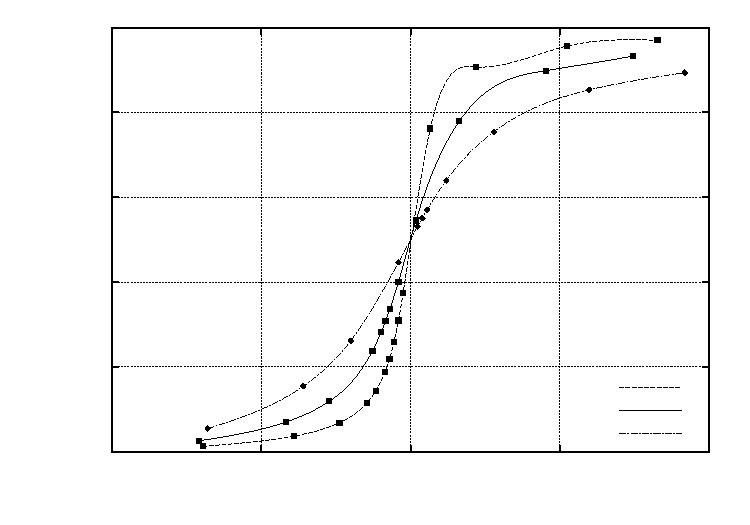
\includegraphics{phasenverschiebung}}%
    \gplfronttext
  \end{picture}%
\endgroup

\caption{Die unterschiedlichen Phasenverschiebungen des Rades abhängig vom Verhältnis von Eigenfrequenz zu 
Anregungsfrequenz}{Anmerkung: Durch die Annäherung mit Splines entspricht der Kurvenverlauf teilweise nicht der Theorie} 
\end{figure}
\newpage \ \\
Aus Abb. \ref{img:2} lassen sich die gemessenen Resonanzfrequenzen bestimmen. Die theoretisch erwarteten Resonanzfrequenzen lassen sich aus den gemessenen Dämpfungskonstanten und Eigenfrequenzen über die Formel
\begin{align}
\omega_r = \sqrt{\omega_0^{2} - 2\beta^{2}} \nonumber
\end{align}
berechnen. Der Vergleich in Tab. \ref{tab:2} zeigt, dass die Werte im Rahmen der Fehlergenauigkeit übereinstimmen. Dies liegt zum Teil auch an den relativ großen Fehlern der berechneten Werte, welche aus der Bestimmung des Logarithmischen Dekrements resultieren. Auffällig ist, dass die erwarteten Werte mit zunehmender Dämpfung tendenziell abfallen, während die gemessenen Werte tendenziell größer werden. 
\begin{table}[!htbp]
\centering
\begin{tabular}{|c|c|c|}
\hline 
Stellung der Wirbelstrombremse & $\omega_r$ erwartet & $\omega_r$ gemessen \\ 
\hline 
$\SI{4}{mm}$ & $\SI{2.1\pm0.4}{\per\second}$ & $\SI{1.95\pm0.10}{\per\second}$ \\ 
\hline 
$\SI{6}{mm}$ & $\SI{2.1\pm0.4}{\per\second}$ & $\SI{1.98\pm0.13}{\per\second}$ \\ 
\hline 
$\SI{8}{mm}$ & $\SI{1.8\pm0.7}{\per\second}$ & $\SI{2.04\pm0.15}{\per\second}$ \\ 
\hline 
\end{tabular} 
\caption{\small{Vergleich der erwarteten und der gemessenen Resonanzfrequenzen}}
\label{tab:2}
\end{table}
\newpage
\newpage
\section{Fehlerrechnung}
\subsection{Aufnahme der Werte}
Da die Güte der verwendeten Messgeräte nicht bekannt ist, muss der Messfehler geschätzt werden. Der Auslenkungswinkel des Pohlschen Rades wird mit einer Auflösung von $\SI{0,25}{\degree}$ aufgezeichnet, daher wird ein Fehler von $\sigma_\varphi=\SI{0,125}{\degree}$ angenommen.

\subsection{Logarithmisches Dekrement}
Der Fehler bei der Berechnung des Logarithmischen Dekrements lässt sich durch eine Gaußsche Fehlerfortpflanzung ermitteln:

\begin{align}
\sigma_\Lambda=\sqrt{\sigma_{\varphi_k}^2\cdot\left( \frac{1}{\varphi_k}\right)^2+\sigma_{\varphi_{k+1}}^2\cdot\left( \frac{1}{\varphi_{k+1}}\right) ^2}
\end{align}
Da die Werte gemittelt werden, wird jeweils der größte Fehler angenommen.
\ \\
Mit einer weiteren Fehlerfortpflanzung folgt der Fehler der Dämpfungskonstante $\beta$

\begin{align}
\sigma_\beta=\sqrt{\sigma_\Lambda^2}
\end{align}

\subsection{Eigenfrequenz}
Der Fehlerfortpflanzung der ungedämpften Eigenfrequenz lautet
\begin{align}
\sigma_{\omega_0} = \sqrt{\sigma_{\omega_e}^{2}\left(\frac{\omega_e}{\sqrt{\omega_e^{2}+\beta^{2}}}\right)^{2}+\sigma_\beta^{2}\left(\frac{\beta}{\sqrt{\omega_e^{2}+\beta^{2}}}\right)^{2}}
\end{align}

\subsection{Resonanzfrequenz}
Die Gaußsche Fehlerfortpflanzung ergibt für die Resonanzfrequenz einen Fehler von
\begin{align}
\sigma_{\omega_r}=\sqrt{\sigma_{\omega_0}\frac{\omega_e}{\sqrt{\omega_e^{2}-2\beta^{2}}}+\sigma_\beta\frac{2\beta}{\sqrt{\omega_e^{2}-2\beta^{2}}}}
\end{align}

\subsection{Diskrete Fouriertransformation}
Die DFT besitzt nur eine begrenzte Auflösung, die von der Anzahl der Messwerte $N$ und der Abtastzeit $t_a$ abhängt. Die Auflösung x berechnet sich zu
\begin{align}
x = \frac{1}{N t_a}
\end{align}
Zu den Frequenzen der DFT addiert sich somit ein Fehler in der Größe der halben Auflösung. In diesem Versuch ist $t_a = \SI{15,625}{ms}$.
\newpage
\section{Diskussion}
Insgesamt war es spannend einen solchen Schwingungsprozess nochmal nachzuvollziehen und auszuwerten. Etwas erfolgreichere
Messergebnisse hätten allerdings die Motivation noch gesteigert.

\subsection{Fehlerdiskussion}
Da eventuelle Ungenauigkeiten bei der Aufnahme der Daten nicht angegeben waren, haben wir uns an der Auflösung 
der aufgezeichneten Daten orientiert, hierbei sind wir von einer \glqq fehlerfreien \grqq{} Zeitbestimmung 
ausgegangen. 
Der wesentlichste vermeidbare Fehler war gegebenenfalls zu kurzes Warten bei der Einschwingzeit, was
die Messergebnisse verfälscht haben kann. \\
Deutlich hat sicherlich der Zustand der Versuchsapparatur zu Fehlern beigetragen, was insbesondere an signifikant 
unterschiedlichen Messergebnissen an den drei Apparaturen zu sehen ist.
Auch die Tatsache dass auch bei kleinster Dämpfung die Amplitude der erzwungenen Schwingung nicht in die Nähe einer 
Resonanzkatastrophe kam spricht für Ungenauigkeiten durch Verschleiß der Apparaturen. \\
Bei der Auswertung der Messwerte hätte man die Fehler beim Logarithmischen Dekrement (sowie den davon abhängigen Werten) minimieren können, indem man weniger Maxima einbezogen (der Fehler nimmt mit kleinerer Amplitude zu) oder ein gewichtetes Mittel verwendet hätte. \\
Eine weitere Auffälligkeit ist die Verschiebung der Resonanzkurven (vgl. Abb. \ref{img:2}). Vor allem die Kurve der starken Dämpfung ist deutlich nach rechts verschoben. Die Ursache dafür könnte entweder im Verschleiß des Messaufbaus oder in der Ungenauigkeit bei der Bestimmung der Eigenfrequenz liegen. Möglicherweise ist auch die Angabe der Exzenterfrequenzen fehlerbehaftet.
\newpage
\thispagestyle{empty}
% Festlegung Art der Zitierung - Havardmethode: Abkuerzung Autor + Jahr
\bibliographystyle{plain}
\bibliography{litbank}{}
\end{document}